\subsection{Wykonywanie SQL przy wywołaniu punktu końcowego}

Wykonywanie SQL przy wywołaniu punktu końcowego to najbardziej skomplikowana
logicznie funkcja programu. Algorytmy są napisane w metodach struktury danych
\verb|EndpointExecutionRuntime|. Definicja struktury danych jest widoczna na
listingu \ref{executionMapListing}. 

Zmienna \verb|request_map| przechowuje dane pobrane z zapytania HTTP. Są
pobierane za pomocą odniesienia \verb|${req.<nazwa>}| w zapytaniu SQL.

Zmienna \verb|execution_maps| przechowuje stos wyników zapytań nadrzędnych.
Przed wykonaniem zapytań podrzędnych, wynik bieżącego zapytania jest odkładany
na stos przechowywany w tej zmiennej.

Zapytania podrzędne są wykonywane dla każdego rzędu będącego wynikiem bieżącego
zapytania SQL, więc na stosie \verb|execution_maps| przechowywane są dane
wynikowe jednego rzędu.

\lstinputlisting[
    float=h!,
    frame=tb,
    label={executionMapListing},
    caption={Struktura danych, której metody wykonują SQL przy wywołaniu punktu
    końcowego}
]{./code/executionMap.rs}

Algorytm znajdowania wartości zmiennej można opisać następująco:

\begin{enumerate}

    \item Jeśli nazwa zaczyna się od ``\verb|req.|'', pobierz z danych z zapytania HTTP,

    \item Jeśli nazwa zaczyna się od ``\verb|super.|'',

        \begin{enumerate}

            \item Ustaw index na rozmiar stosu tablic wynikowych operacji nadrzędnych,

            \item Dopóki nazwa zaczyna się od ``\verb|super.|'',

                \begin{enumerate}

                    \item Zmniejsz indeks o 1,

                    \item Usuń ``\verb|super.|'' z początku nazwy zmiennej,

                \end{enumerate}

            \item Pobierz wartość z tablicy mieszającej ze stosu pod wynikowym
                indeksem, gdzie klucz jest równy nazwie zmiennej.

        \end{enumerate}

\end{enumerate}

Implementacja algorytmu została zamieszczona na listingu
\ref{findingVariablesListing}. Diagram obrazujący działanie algorytmu
przedstawiono na rysunku \ref{variableResolutionFigure}.

\lstinputlisting[
    basicstyle=\footnotesize\ttfamily,
    float=h!,
    frame=tb,
    label={findingVariablesListing},
    caption={Algorytm znajdowania wartości zmiennej}
]{./code/findingVariables.rs}

\begin{figure}[h]
    \centering
    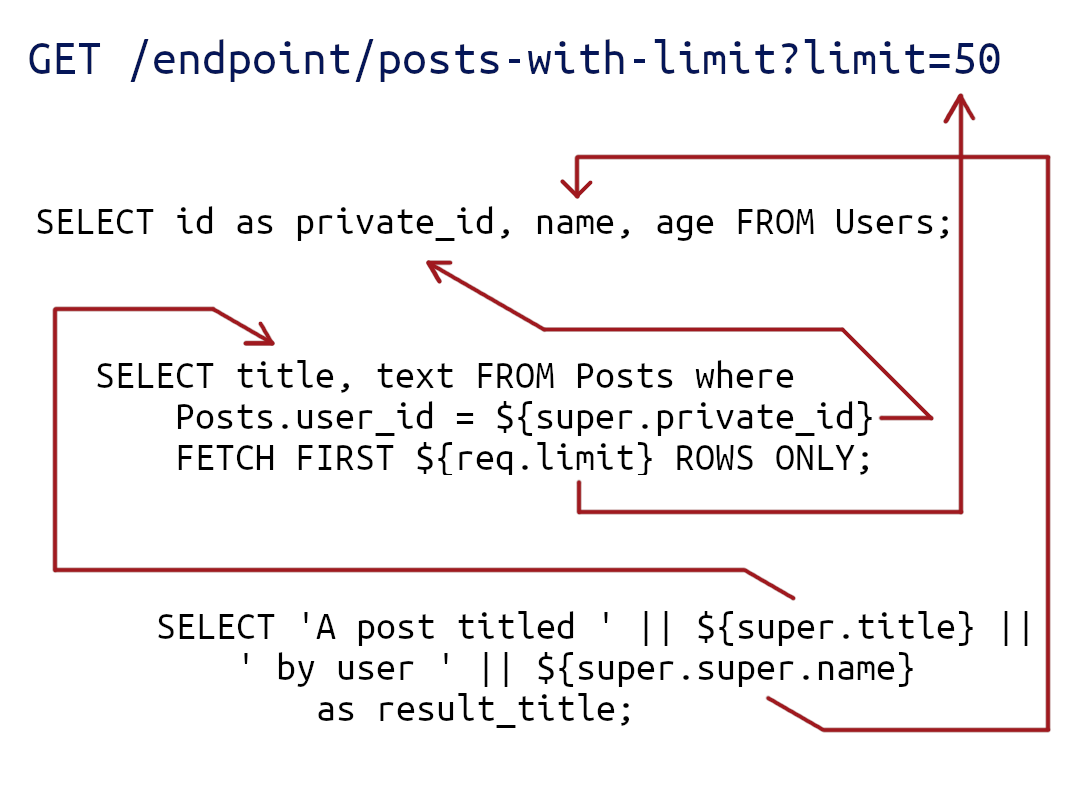
\includegraphics[width=0.7\textwidth]{./img/variable_resolution.png}
    \caption{Diagram obrazujący działanie algorytmu znajdowania wartości zmiennych}
    \label{variableResolutionFigure}
\end{figure}

Algorytm wykonywania drzewa zapytań SQL można opisać następująco:

\begin{enumerate}

    \item Dla każdego zapytania SQL przypisanego do punktu końcowego,

        \begin{enumerate}

            \item Dla każdego argumentu pobieranego przez zapytanie,

                \begin{enumerate}

                    \item Pobierz wartość argumentu z zapytania HTTP lub wyników
                        zapytań nadrzędnych,

                    \item Wykonaj zapytanie SQL na bazie danych,

                    \item Dla każdego wiersza, który zwróci baza danych, zapisz
                        kolumny w tablicy mieszającej,

                        \begin{enumerate}

                            \item Odłóż wynikową tablicę na stos,

                            \item Rekurencyjnie wywołaj algorytm dla zapytań
                                podrzędnych,

                        \end{enumerate}

                \end{enumerate}

        \end{enumerate}

\end{enumerate}

Całość algorytmu jest wykonywana z użyciem asynchronicznego dostępu do bazy
danych.

Implementacja algorytmu została zamieszczona na listingu
\ref{endpointExecutionListing}.

\clearpage

\lstinputlisting[
    basicstyle=\footnotesize\ttfamily,
    frame=tb,
    label={endpointExecutionListing},
    caption={Algorytm wykonywania drzewa zapytań SQL}
]{./code/endpointExecution.rs}
